\chapter{Learning to reason with LLMs}
\label{chap:lec02_learning_to_reason}
\section{本讲学习目标}

第二讲把课程焦点从“推理时怎么花预算”转向“如何把 reasoning 行为直接教给模型”。Jason Weston 的核心论点是：如果我们只把语言模型当成会模仿文本的 System 1，那么它会持续暴露出 hallucination、sycophancy、jailbreaking 等模式匹配型失败；真正困难的地方在于，\textbf{如何让模型既会回答，也会评价回答，从而形成自我改进的闭环。}

读完本讲后，读者应能回答：
\begin{itemize}
\item 为什么 Weston 把 reasoning learning 的问题重写成“如何得到更可靠的 judgments / rewards”。
\item SFT、RLHF、DPO 在 post-training 谱系中各自扮演什么角色，为什么 DPO 会成为讲者首选的训练积木。
\item CoVe、System 2 Attention、Branch-Solve-Merge 这些方法如何把“长一点的思考”改写成“显式验证与分解”。
\item Self-Rewarding LM、IRPO、Thinking LLMs、Meta-Rewarding、EvalPlanner 之间的递进关系是什么。
\item 为什么 reasoning 训练最难的往往不是 actor，而是 evaluator / judge。
\end{itemize}

\section{背景与问题设置}

\subsection{把“学习推理”看成学习更好的 judge}

Weston 一开场就把目标说得很尖锐：理想 AI 应该尽可能\textbf{自己给自己出题、自己判断做得好不好、再根据这些判断继续更新自己。} 这不是简单自动化，而是在追问一个更基础的问题：当模型能力越来越接近甚至超过普通人时，谁来继续稳定地给它提供训练信号？

\begin{figure}[H]
\centering
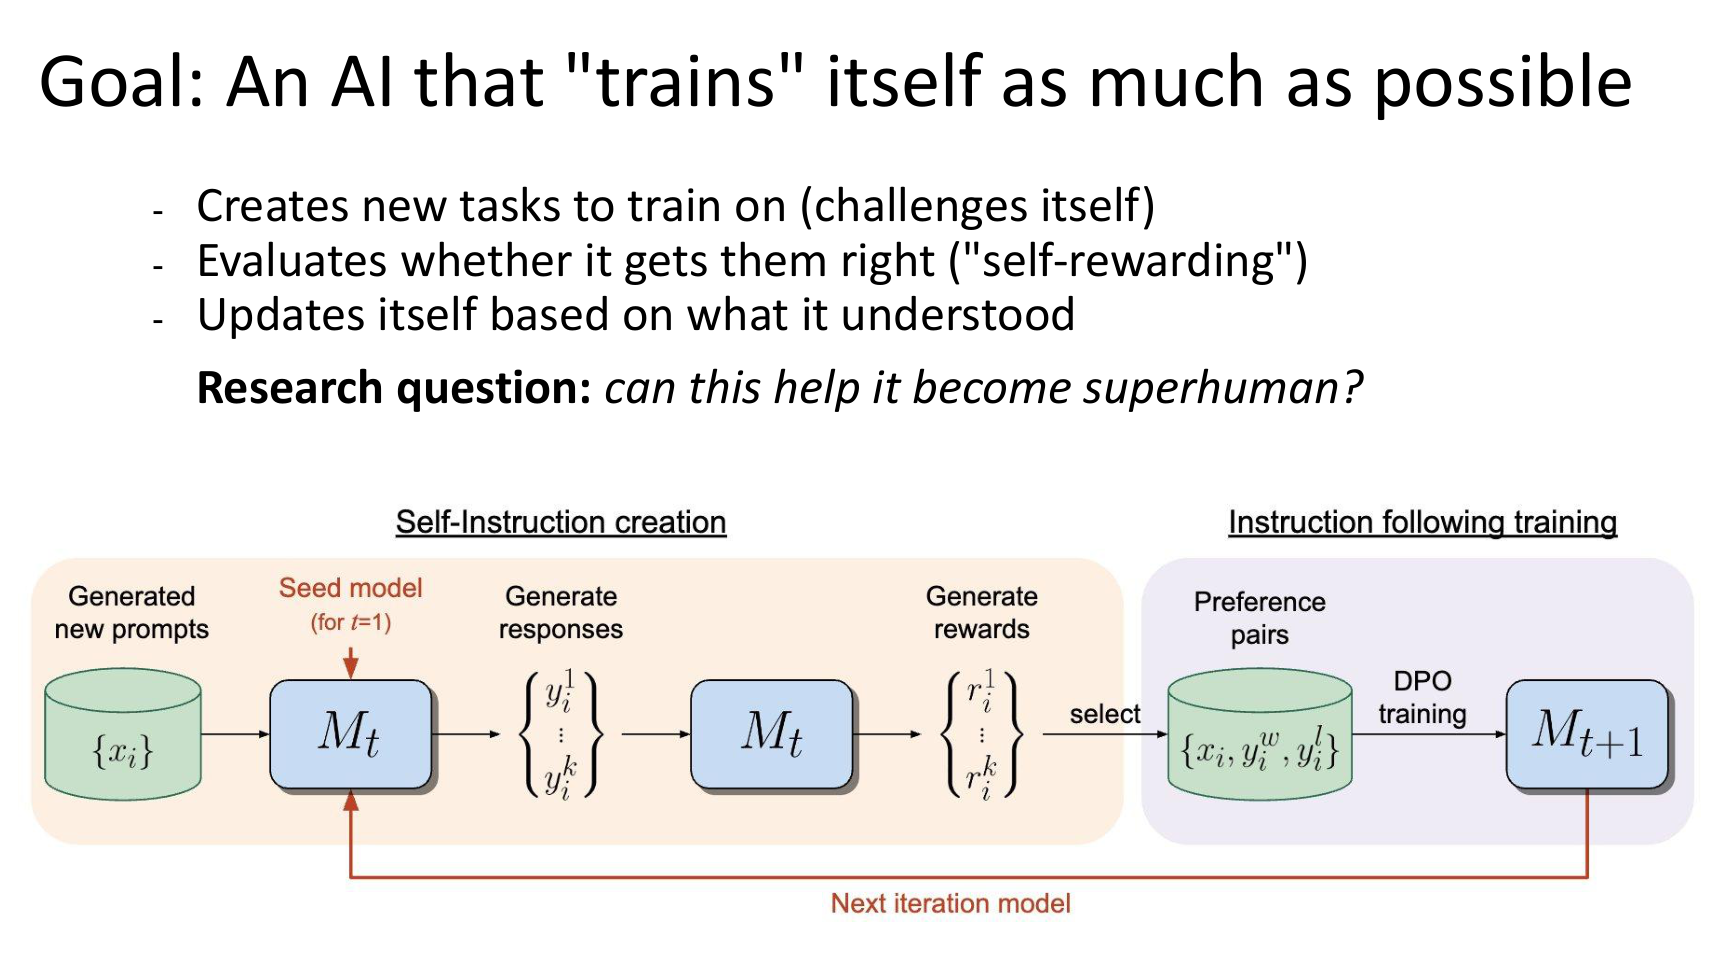
\includegraphics[width=0.82\textwidth]{../lectures/lec02_learning_to_reason/figures/lec02_fig_001.png}
\caption{Weston 对 self-training AI 的定义：能生成任务、分配 reward、并把这些 judgments 重新喂回训练流程。}
\end{figure}

这一定义已经隐含了本讲的中心思想。Reasoning 不仅是“生成更长的 chain-of-thought”，而是：\textbf{模型能否获得足够高质量的反馈信号，判断哪条思路更好、哪条思路只是看起来像思考。}

\subsection{System 1 失败为什么逼着我们走向 System 2}

在 Weston 的叙述里，当前 LLM 更像 \textbf{System 1}：反应快、擅长联想、每个 token 都是固定计算，但很容易学到不该学的相关性。幻觉、迎合用户错误观点、越狱，本质上都是“反应式模式匹配”超出安全工作区后的副产物。换句话说，问题不只是模型会错，而是它经常\textbf{没有显式的机制停下来检查自己。}

Weston 因此把 reasoning 引向了一个很务实的方向：与其要求模型凭空更聪明，不如先让它学会更系统地\textbf{验证（verification）、重写（rewriting）、分解（decomposition）和评价（judging）}。这就是他所说的 System 2 路线。

\subsection{后训练谱系：SFT、RLHF、DPO}

在进入 reasoning-specific 方法之前，讲者先回顾 pre-o1/r1 时代的 post-training 谱系：SFT 用任务示例继续做 next-token learning，RLHF 引入人类偏好与 reward model，而 DPO 则把 RLHF 的目标改写成一个更稳定直接的 preference optimization loss。

\begin{figure}[H]
\centering
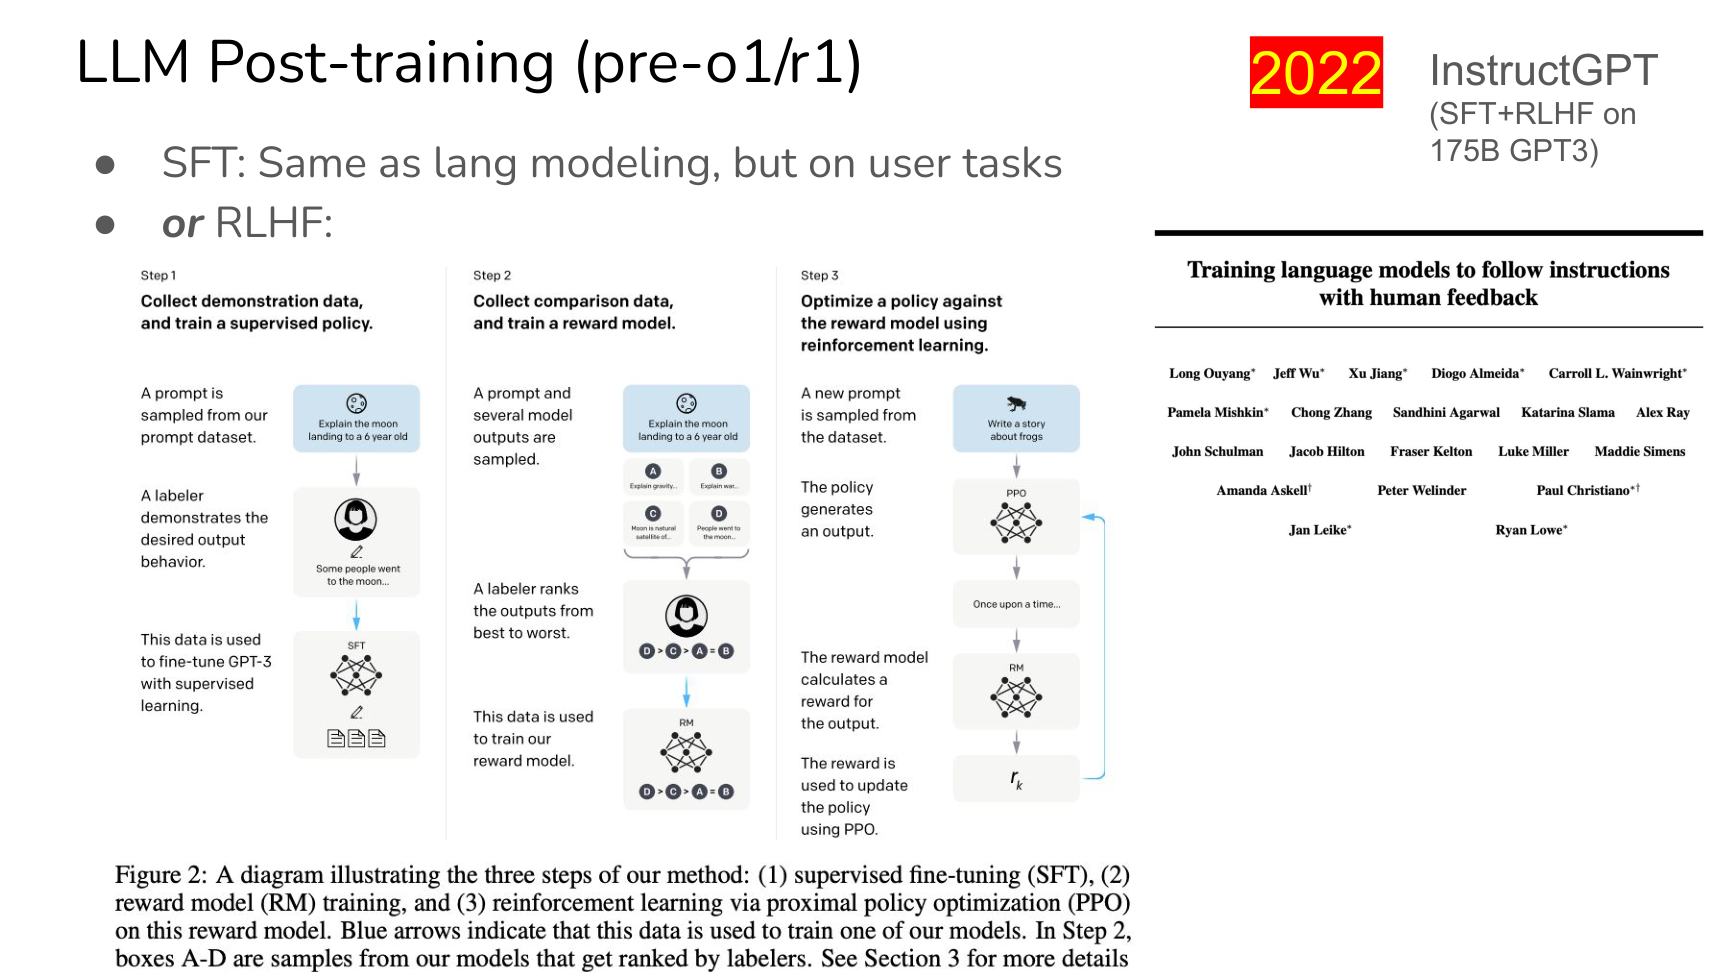
\includegraphics[width=0.80\textwidth]{../lectures/lec02_learning_to_reason/figures/lec02_fig_002.png}
\caption{SFT、RLHF、DPO 构成 Weston 后续所有训练 recipe 的基本骨架。}
\end{figure}

DPO 的标准写法是：
\[
\mathcal{L}_{\mathrm{DPO}}(\theta)=-\mathbb{E}_{(x,y_w,y_l)}\left[\log \sigma\left(\beta \log \frac{\pi_\theta(y_w \mid x)}{\pi_{\mathrm{ref}}(y_w \mid x)}-\beta \log \frac{\pi_\theta(y_l \mid x)}{\pi_{\mathrm{ref}}(y_l \mid x)}\right)\right]
\]
其中 $\pi_\theta$ 是要训练的模型，$\pi_{\mathrm{ref}}$ 是参考模型，$x$ 是输入指令，$y_w$ 与 $y_l$ 分别是胜出和败北回答，$\beta$ 控制偏离参考模型的强度。直觉上，DPO 不再单独训练一个 reward model 再跑 RL，而是直接把“更喜欢 $y_w$ 而不是 $y_l$”写进模型更新目标。

\begin{importantbox}{这条公式为什么重要}
Weston 之后讲的 self-rewarding、IRPO、meta-rewarding 都要回到同一个问题：\emph{偏好对从哪来？} DPO 本身不是答案，它只是一个非常好用的“执行器”。真正困难的是如何构造足够可信的 $(y_w, y_l)$。
\end{importantbox}

\section{主体讲解}

\subsection{先把验证这件事做清楚：CoVe、System 2 Attention、Branch-Solve-Merge}

\subsubsection{Chain-of-Verification：不是更长 CoT，而是更可审计的 CoT}

CoVe 的贡献在于，它把“再想一遍”拆成四个可解释的步骤：先给草稿答案，再生成 verification questions，然后独立回答这些问题，最后整合成最终答案。

\begin{figure}[H]
\centering
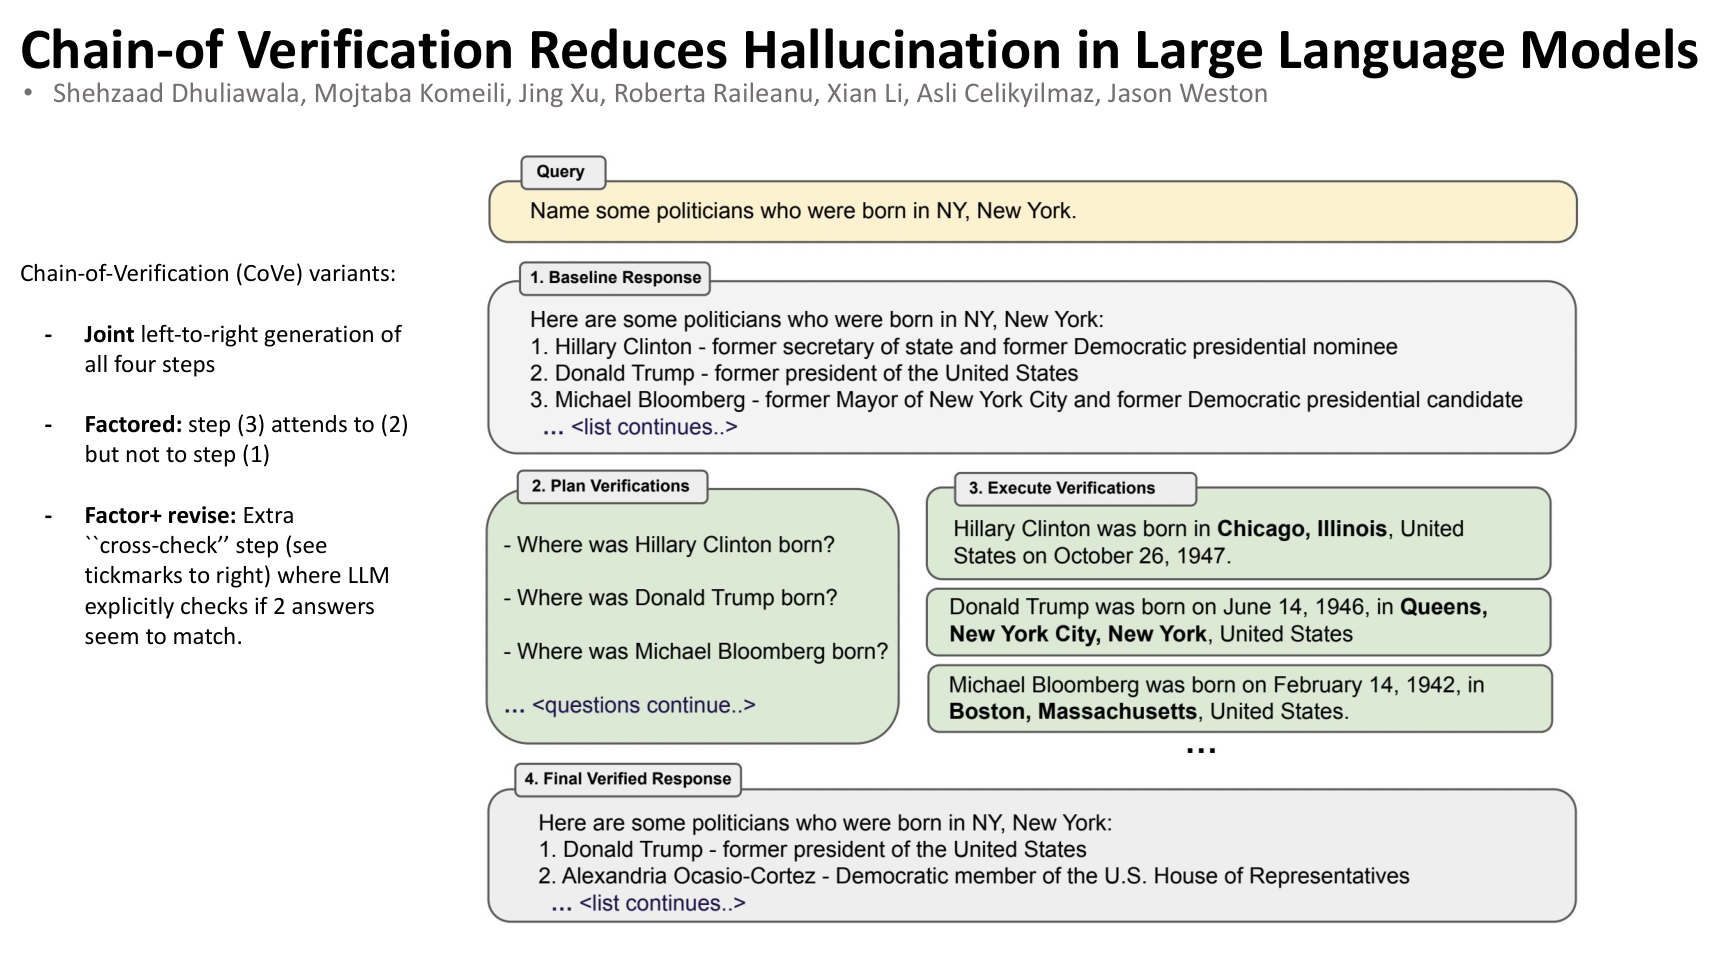
\includegraphics[width=0.78\textwidth]{../lectures/lec02_learning_to_reason/figures/lec02_fig_003.png}
\caption{CoVe 把验证流程显式拆解，核心目的是减少最终回答对原始错误草稿的路径依赖。}
\end{figure}

\begin{lstlisting}
Draft an initial answer
Plan verification questions
Answer each verification question independently
Synthesize a final verified response
\end{lstlisting}

这和第一讲里那种“让模型多采样几条 CoT 再投票”不同。CoVe 面向的是 factuality / hallucination 场景：如果错误来自事实断言，而不是搜索宽度不足，那么更关键的是\textbf{把事实核查环节显式写进流程}。

\paragraph{为什么要独立回答 verification questions}
如果 verification step 继续强依赖原始草稿，那么模型只是在原错误附近做润色。CoVe 要求各验证问题独立作答，目的正是防止 answer contamination。

\subsubsection{System 2 Attention 与 Branch-Solve-Merge}

Weston 随后给出另外两类 System 2 方法。System 2 Attention（S2A）不急着回答，而是先重写问题，尽量移除与任务无关的偏见和干扰项，再基于重写后的问题作答。

\begin{figure}[H]
\centering
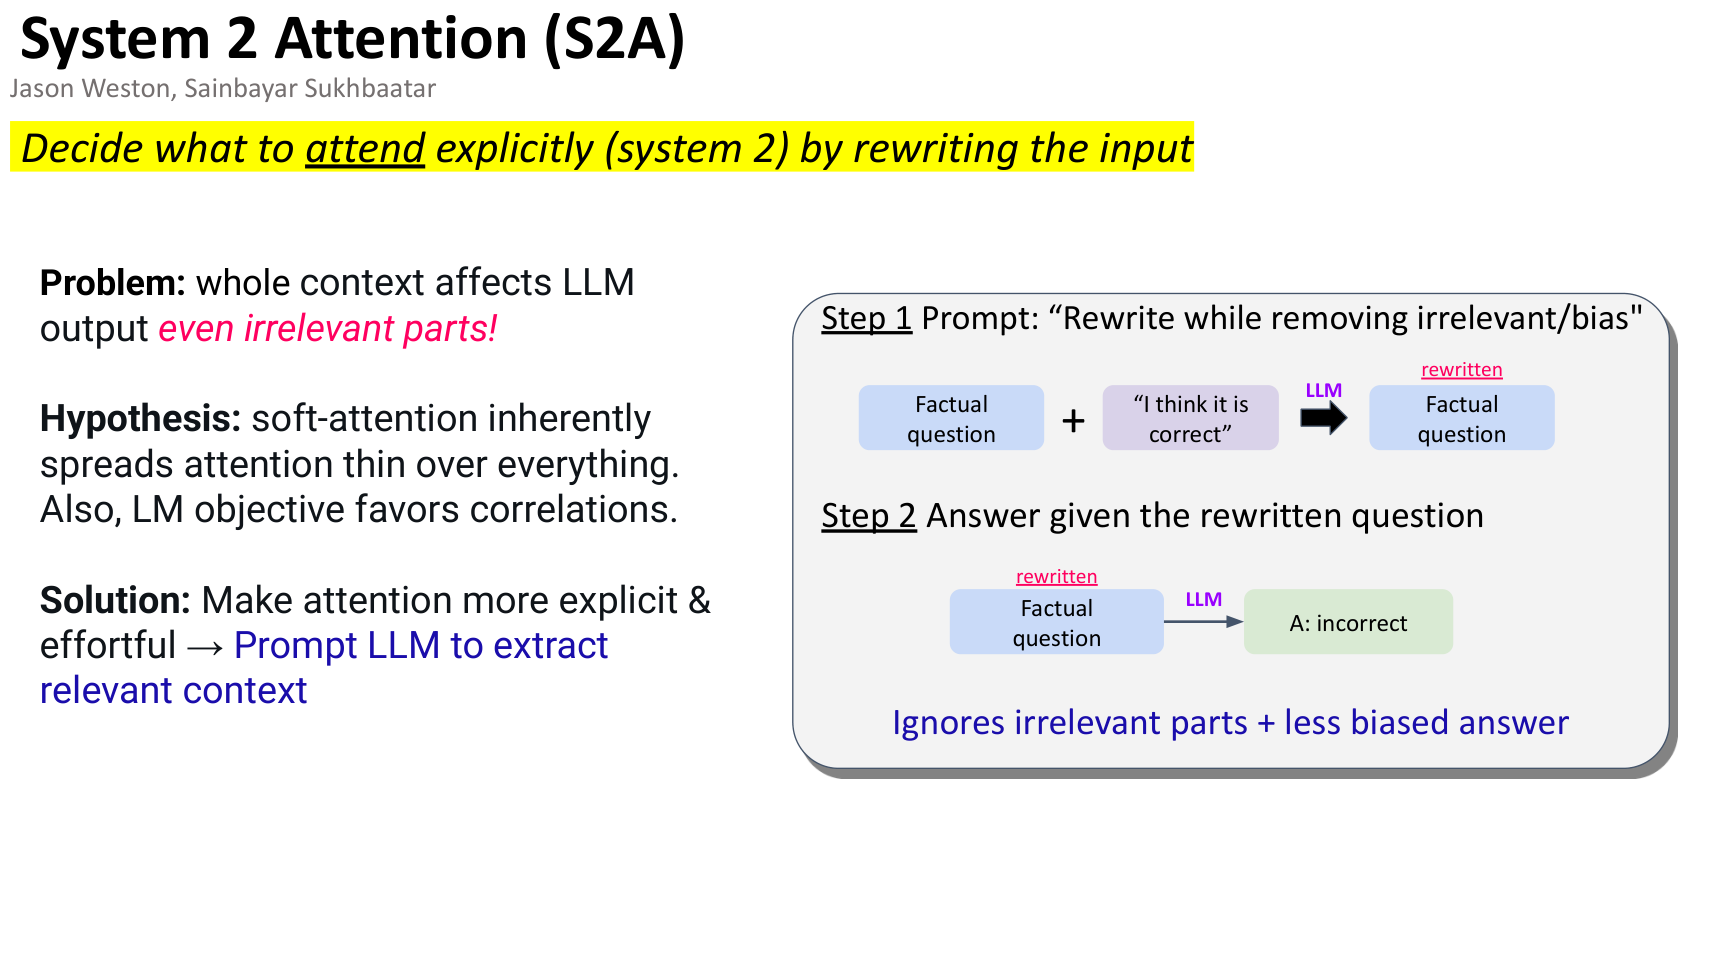
\includegraphics[width=0.80\textwidth]{../lectures/lec02_learning_to_reason/figures/lec02_fig_004.png}
\caption{S2A 的关键是先决定“应该注意什么”，而不是直接在有偏输入上给答案。}
\end{figure}

这背后的直觉非常实用：不少 hallucination 不是知识完全缺失，而是模型注意力被噪声、用户偏见或表述方式带偏了。S2A 先做 \textbf{attention selection}，再做 answering。

Branch-Solve-Merge 则把复杂评价或生成任务拆成多个子问题，分别求解后再融合。它更像“评估任务也需要 planning”。和第一讲的 Tree of Thoughts 很像，只是这里的对象更多是\textbf{response evaluation} 而不是 search over candidate answers。

\begin{knowledgebox}{本节的统一主线}
Weston 给出的 System 2 方法有一个共同点：它们都把“多花一点 token”变成了“对哪一步花 token、为什么花 token”的结构化决策。
\end{knowledgebox}

\subsection{Self-Rewarding：为什么 reasoning learning 会卡在 human bottleneck}

\subsubsection{标准 RLHF 的扩展瓶颈}

当模型还不强时，人类给偏好标签并不太困难；一旦回答很长、主题专业、甚至模型在某些方面超过普通评审，人类就会越来越难稳定判断“哪个更好”。

\begin{figure}[H]
\centering
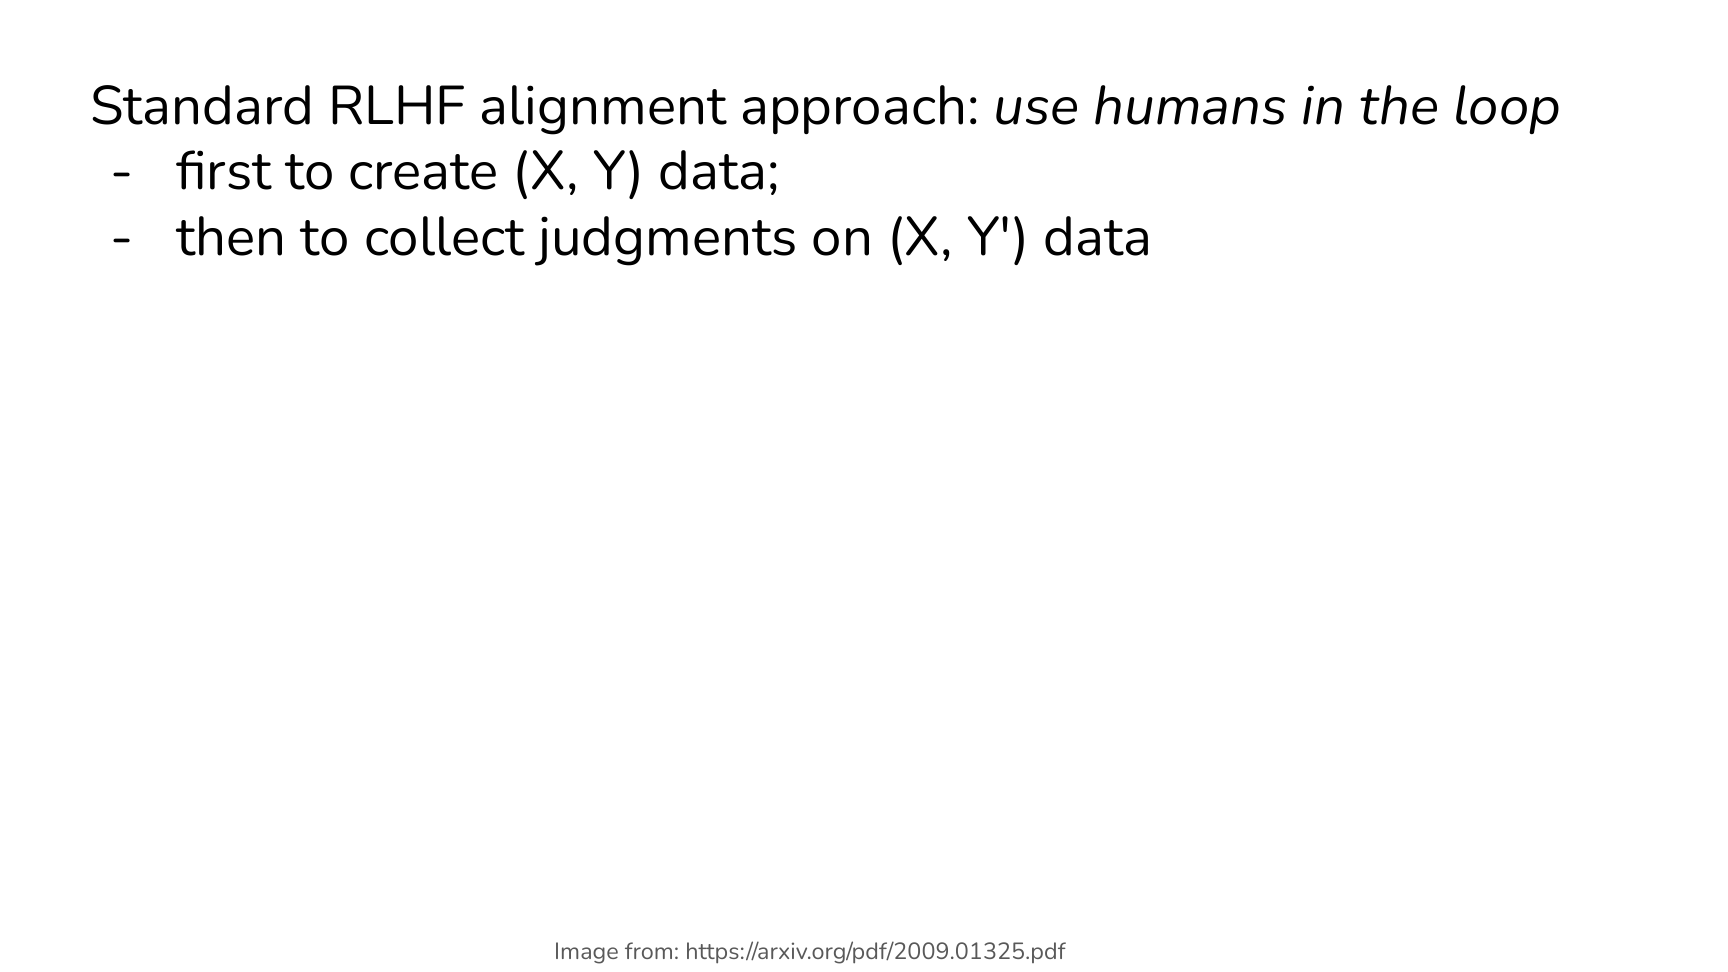
\includegraphics[width=0.74\textwidth]{../lectures/lec02_learning_to_reason/figures/lec02_fig_005.png}
\caption{标准 RLHF 把人类放在数据生产和偏好判断两个关键位置，因此扩展能力直接受限于人类评审吞吐量。}
\end{figure}

Weston 的研究问题很明确：\textbf{如果继续提升模型需要更高质量的 judgments，而 humans in the loop 已经成为瓶颈，那么能不能让模型学习生成这些 judgments？}

\subsubsection{Self-Rewarding LM：actor 和 judge 双能力模型}

Self-rewarding LM 的定义不是“模型给自己打分”这么简单。Weston 强调它至少要有两种能力：
\begin{itemize}
\item \textbf{instruction following capability}：能对用户指令给出较好回答。
\item \textbf{evaluation capability}：能区分更好和更差的回答，并给出可用的偏好信号。
\end{itemize}

\begin{figure}[H]
\centering
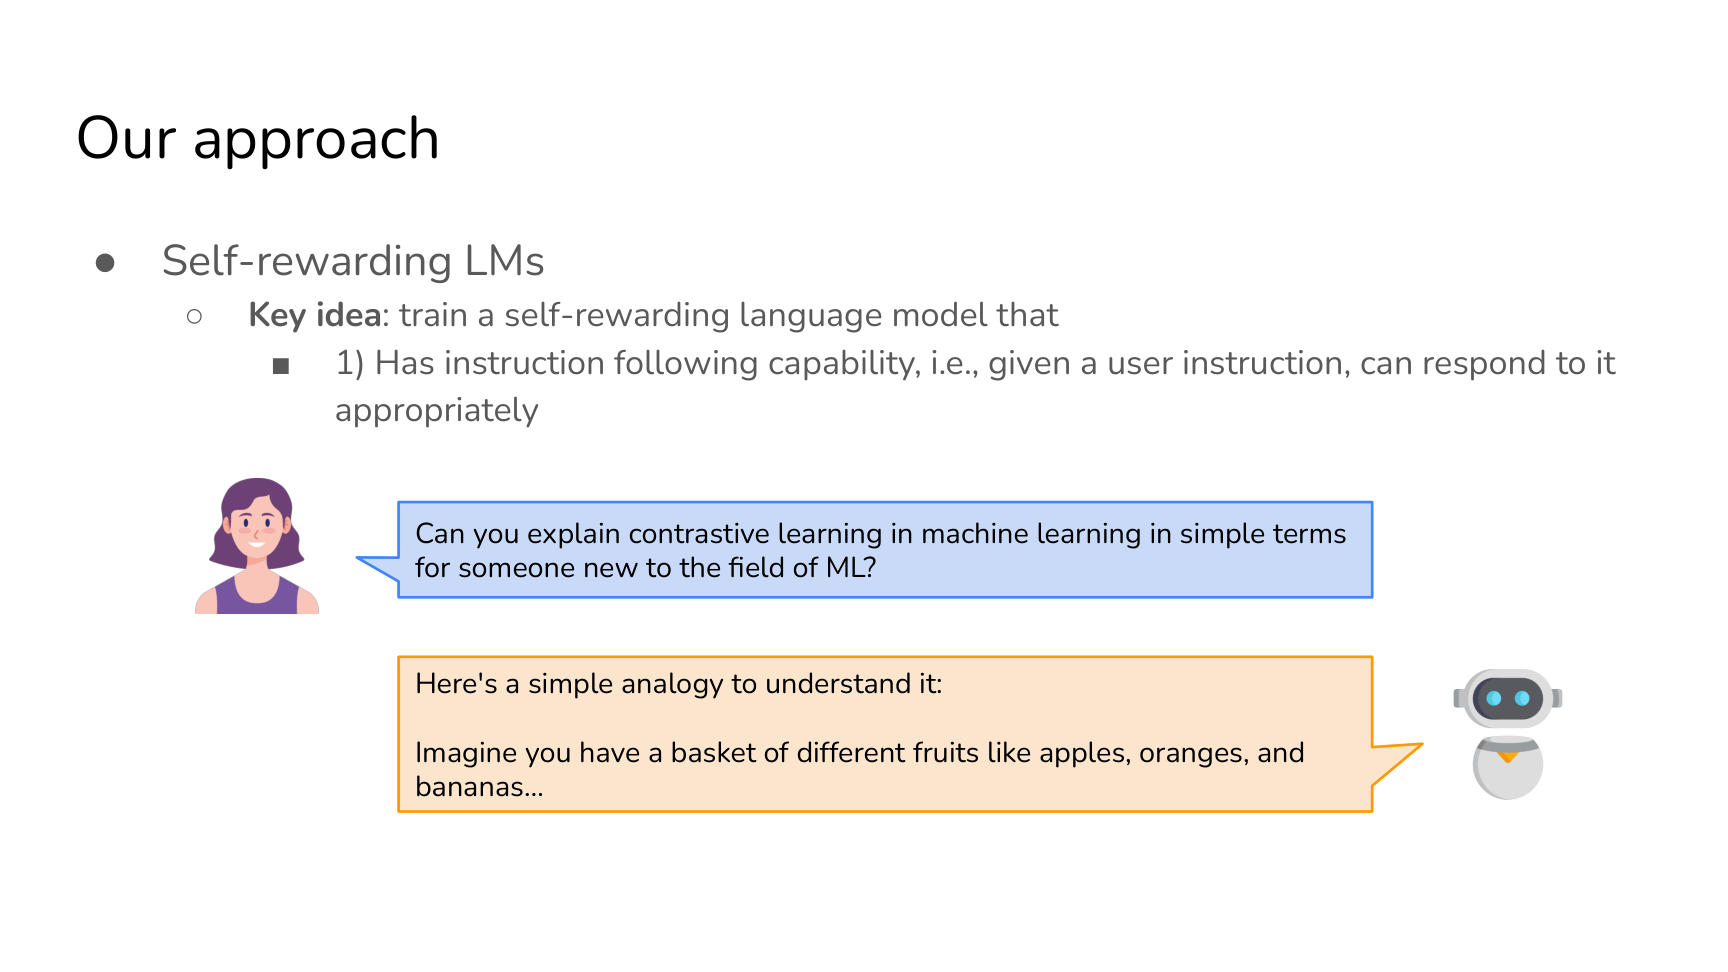
\includegraphics[width=0.76\textwidth]{../lectures/lec02_learning_to_reason/figures/lec02_fig_006.png}
\caption{Self-rewarding 模型既是 actor 也是 judge。Weston 的关键不是“省人力”，而是让 evaluator 能随着 actor 一起成长。}
\end{figure}

可以用一个极简抽象写成：
\[
\mathcal{D}_{t+1}=\mathcal{D}_{t}\cup\{(x,\{(y_i,r_i)\}_{i=1}^{k})\}
\]
其中 $\mathcal{D}_t$ 是已有数据集，模型对同一指令 $x$ 生成多个回答 $y_i$ 并赋予分数 $r_i$，然后把这些 judged candidates 再变成新的训练材料。

\paragraph{为什么这不是自嗨}
如果模型只会生成、不会评估，那么新的训练数据不过是旧偏差的放大器。Self-rewarding 的真正难点在于 judge 能否提供\textbf{比现有 actor 更可靠的排序}。

\subsubsection{训练 recipe 与实验设计}

Lecture 给出的 recipe 很具体：从一个带少量 seed instruction-following data 和 evaluation data 的模型出发，在每轮中生成 prompts、candidate responses 和 self-rewards，然后把选出的 preference pairs 用 DPO 继续训练。

\begin{figure}[H]
\centering
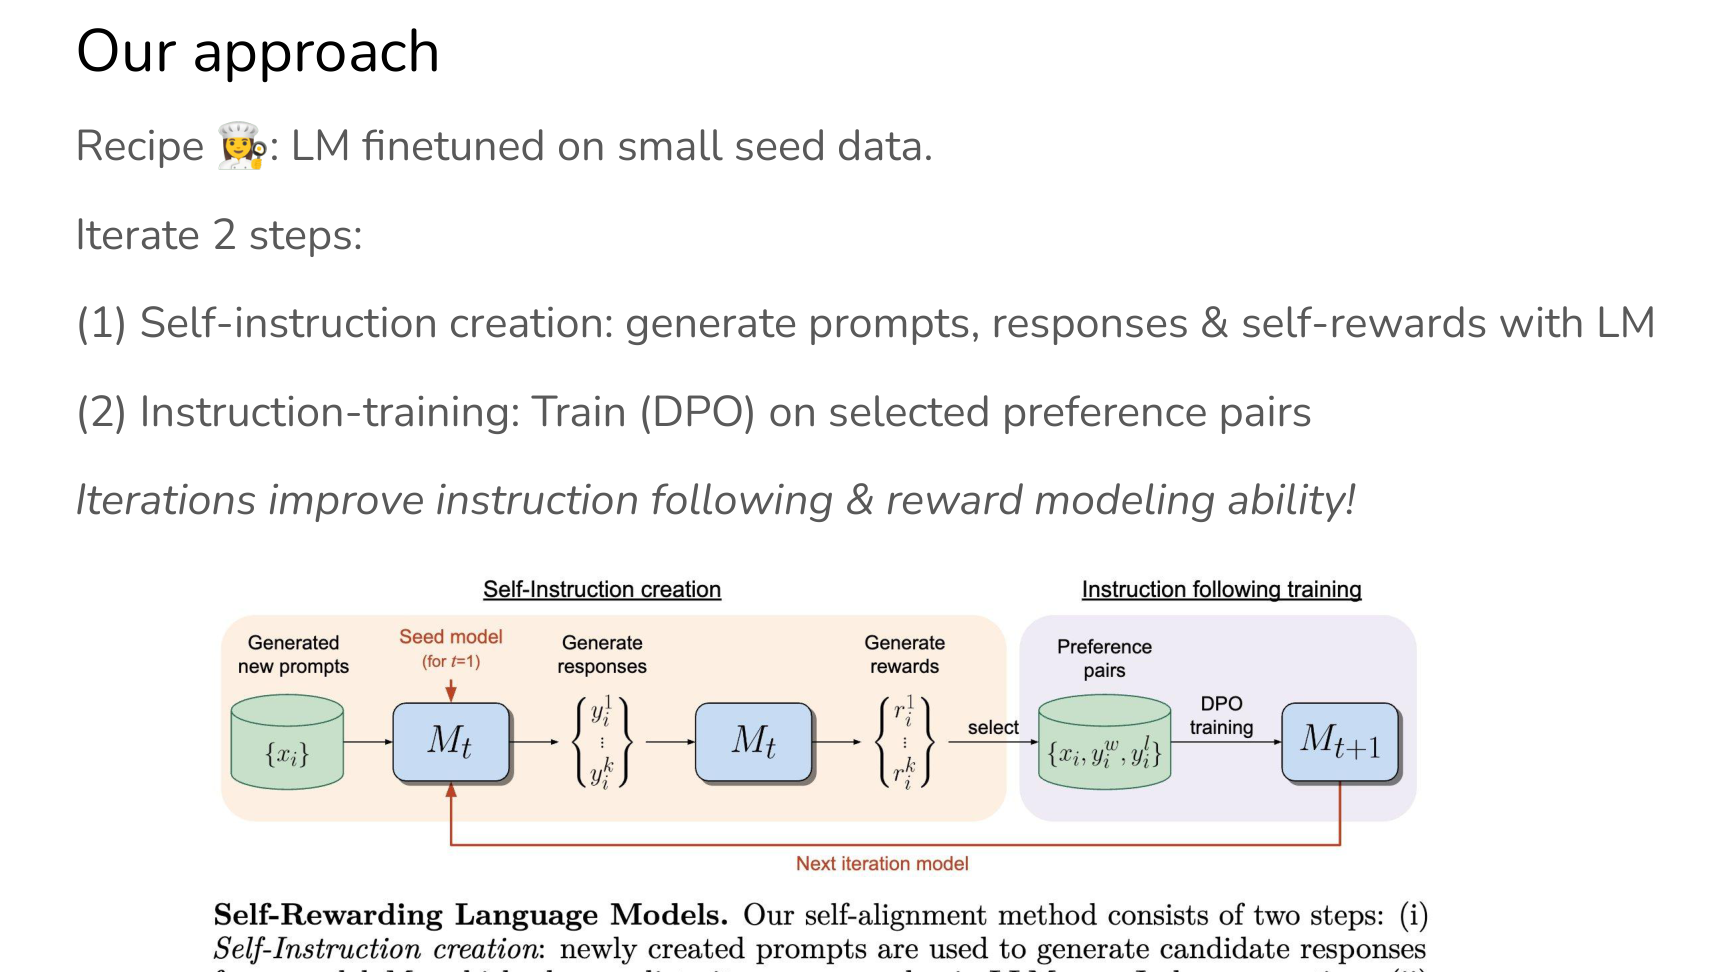
\includegraphics[width=0.78\textwidth]{../lectures/lec02_learning_to_reason/figures/lec02_fig_007.png}
\caption{Self-rewarding 训练 recipe：生成、判断、筛选、DPO，再迭代。}
\end{figure}

\begin{lstlisting}
Initialize M1 with seed instruction-following and evaluation data
For each iteration t:
    generate prompts, candidate responses, and self-rewards with Mt
    select preference pairs from the judged candidates
    run DPO to obtain M(t+1)
\end{lstlisting}

讲者特别展示了 LLM-as-a-Judge prompt 的维度设计：relevance、coverage、usefulness、clarity、expertise。这个细节非常关键，因为 reasoning training 不是只要一个 scalar reward 就够了；如果 reward 的来源不可解释、不可审计，那么后续迭代只会更脆弱。

\begin{figure}[H]
\centering
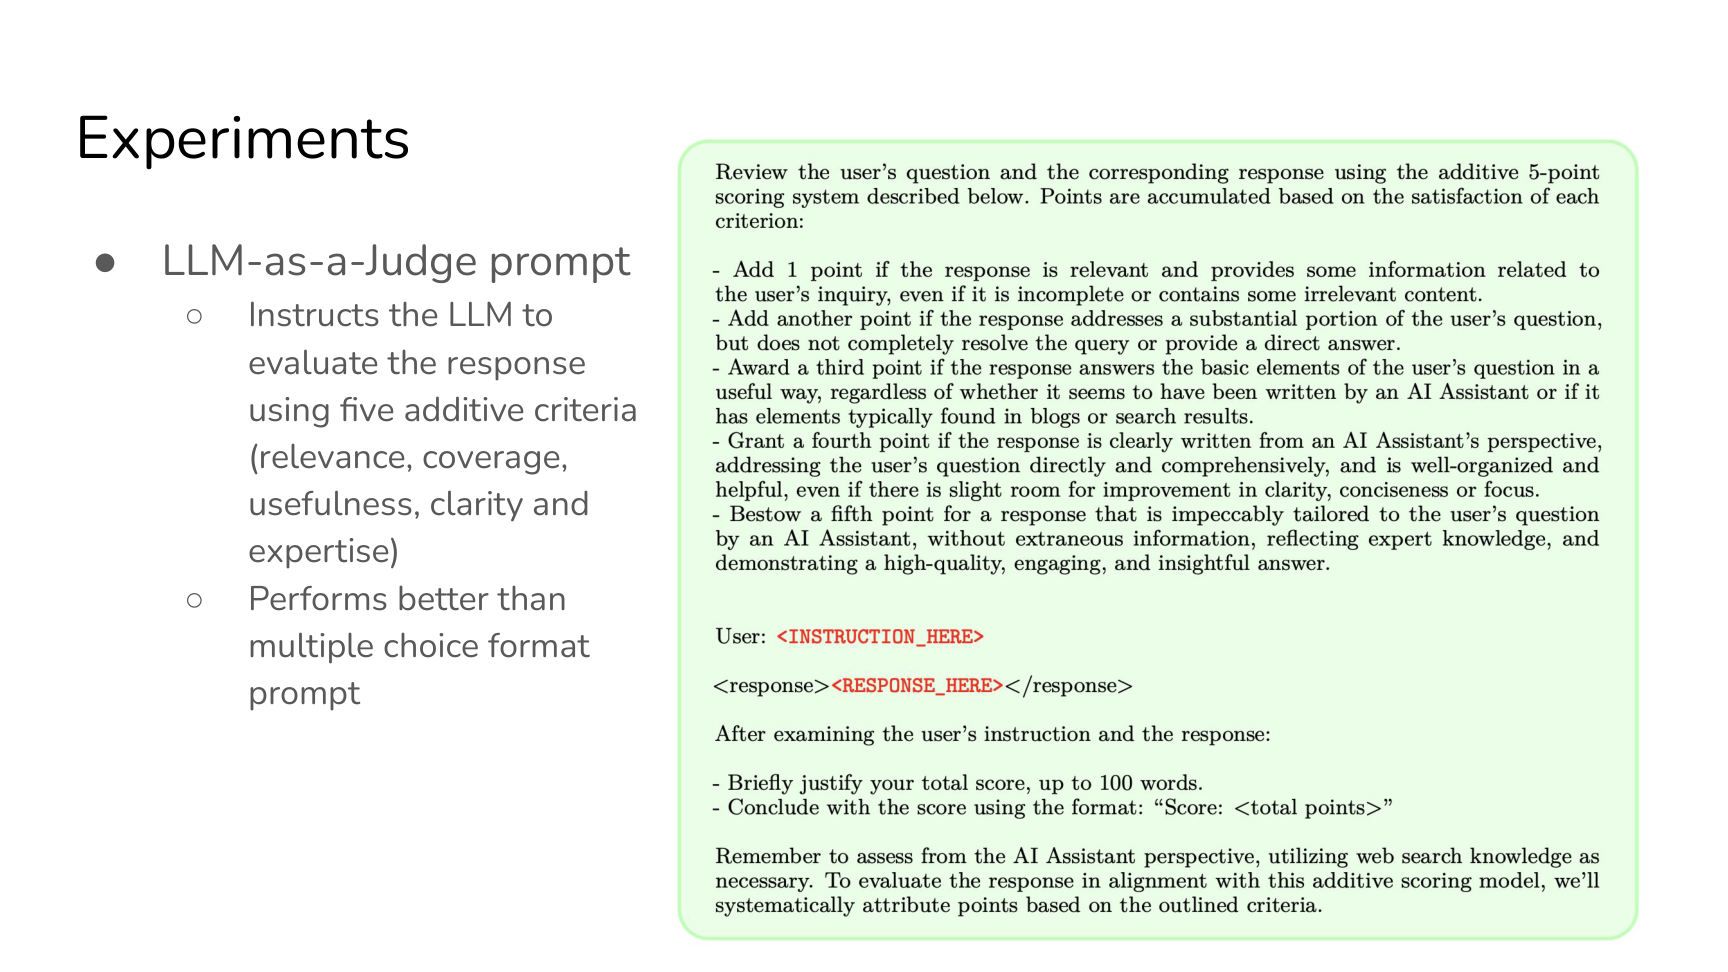
\includegraphics[width=0.78\textwidth]{../lectures/lec02_learning_to_reason/figures/lec02_fig_008.png}
\caption{Weston 强调 judge prompt 要拆解成多个 criteria，避免 evaluator 只学到模糊的“我喜欢这个回答”。}
\end{figure}

\paragraph{实验结果的真正含义}
Self-rewarding 模型在 instruction following 和 reward modeling 两个轴上都持续提升，这说明“学会 judging”不会天然拖累“学会 acting”。但讲者没有把这个结果夸成万能方案，因为 reasoning tasks 仍然比一般 instruction following 更难，需要更强的可验证信号。

\subsection{IRPO：把 preference optimization 从 style alignment 拉回 reasoning}

\subsubsection{为什么 reasoning 需要更强的 reward structure}

Weston 在第一个 self-rewarding 结果之后立刻承认一个限制：模型确实更会回答、也更会评分了，但\textbf{reasoning task 仍然提升有限。} 原因是通用偏好标签更像 style / helpfulness alignment，而 reasoning task 需要对中间思路的成败有更细粒度的 credit assignment。

\begin{figure}[H]
\centering
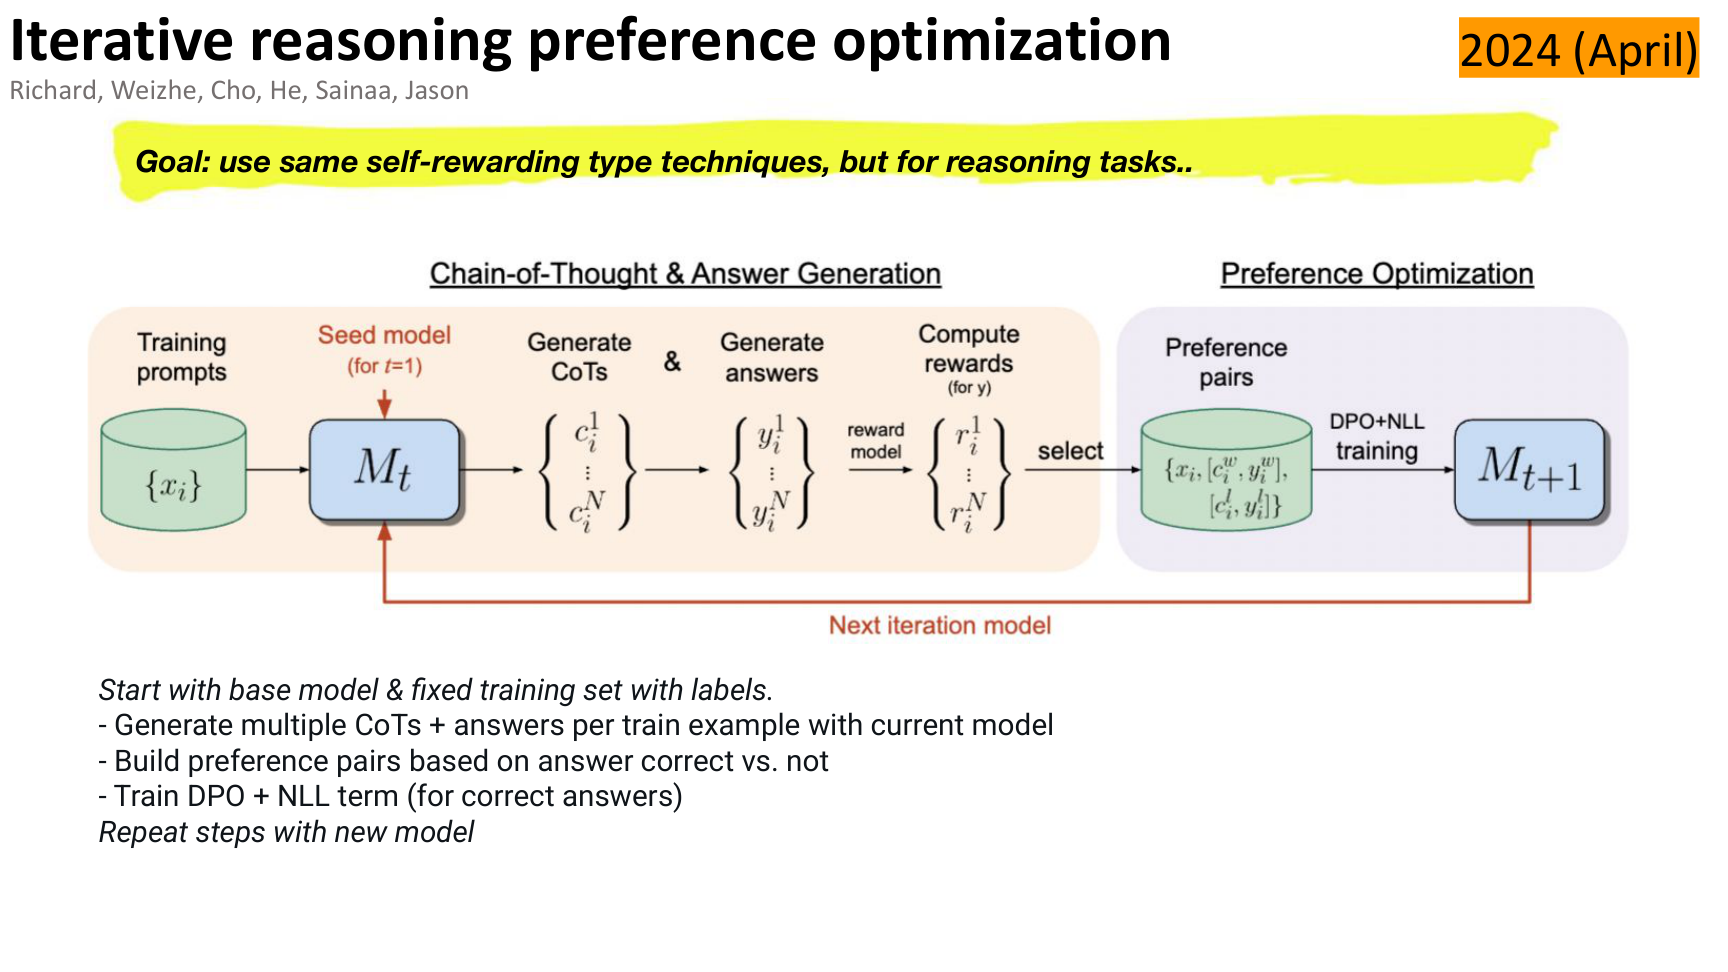
\includegraphics[width=0.78\textwidth]{../lectures/lec02_learning_to_reason/figures/lec02_fig_009.png}
\caption{IRPO 的出发点：reasoning task 需要的不只是好回答，而是“哪条思路最终导致了可验证正确答案”。}
\end{figure}

IRPO 的基本流程是：对每个问题采样多条 chain-of-thought，抽取最终答案，用可验证规则判断最终答案是否正确，再保留那些通向正确 final answer 的 reasoning traces，把它们与失败 traces 组成 preference pairs。

它的目标写成：
\[
\mathcal{L}_{\mathrm{IRPO}}=\mathcal{L}_{\mathrm{DPO}}+\lambda\,\mathcal{L}_{\mathrm{NLL}}(y^{\star}_{\mathrm{cot}})
\]
其中 $\mathcal{L}_{\mathrm{DPO}}$ 负责学习 winning / losing CoT 的相对偏好，$\mathcal{L}_{\mathrm{NLL}}$ 则继续鼓励模型模仿正确 reasoning trace，$y^{\star}_{\mathrm{cot}}$ 表示到达可验证正确 final answer 的那条 CoT。

\begin{lstlisting}
Sample multiple CoT candidates per problem
Extract the final answer from each candidate
Keep trajectories whose final answer is verifiably correct
Create winning/losing reasoning pairs
Train with DPO plus an NLL term on the winning traces
\end{lstlisting}

\paragraph{为什么 negative examples 是关键}
Lecture 明确指出：如果只做 SFT，chosen 和 rejected generations 在 token 级概率上常常被拉得太近，模型无法真正学会“哪种 reasoning style 会通往正确答案”。IRPO 需要明确失败样本，才能把 reasoning 区分开来。

\subsubsection{IRPO 的边界条件}

IRPO 最大的优点是 reward 来自\textbf{可验证 final answer}，这让 reasoning learning 有了更坚实的地基。但它也有明确边界：
\begin{itemize}
\item 任务必须存在可验证答案，至少 final answer 要能自动判对错。
\item 对开放式任务、创造性任务、模糊评价任务，IRPO 的 reward grounding 会变弱。
\item 它仍然是在固定问题集上循环，不等于 agent 已经能在开放环境中自发发现新 reasoning tasks。
\end{itemize}

\subsection{Thinking LLMs、Meta-Rewarding 与 EvalPlanner}

\subsubsection{Thinking LLMs：thought generation 不应只服务数学}

Weston 进一步指出，o1 / R1 式“先想后答”不应该只限于数学或可验证推理。Thinking LLMs / Thought Preference Optimization（TPO）的目标，是让模型在一般 instruction following 任务里也学会 thought generation。

\begin{figure}[H]
\centering
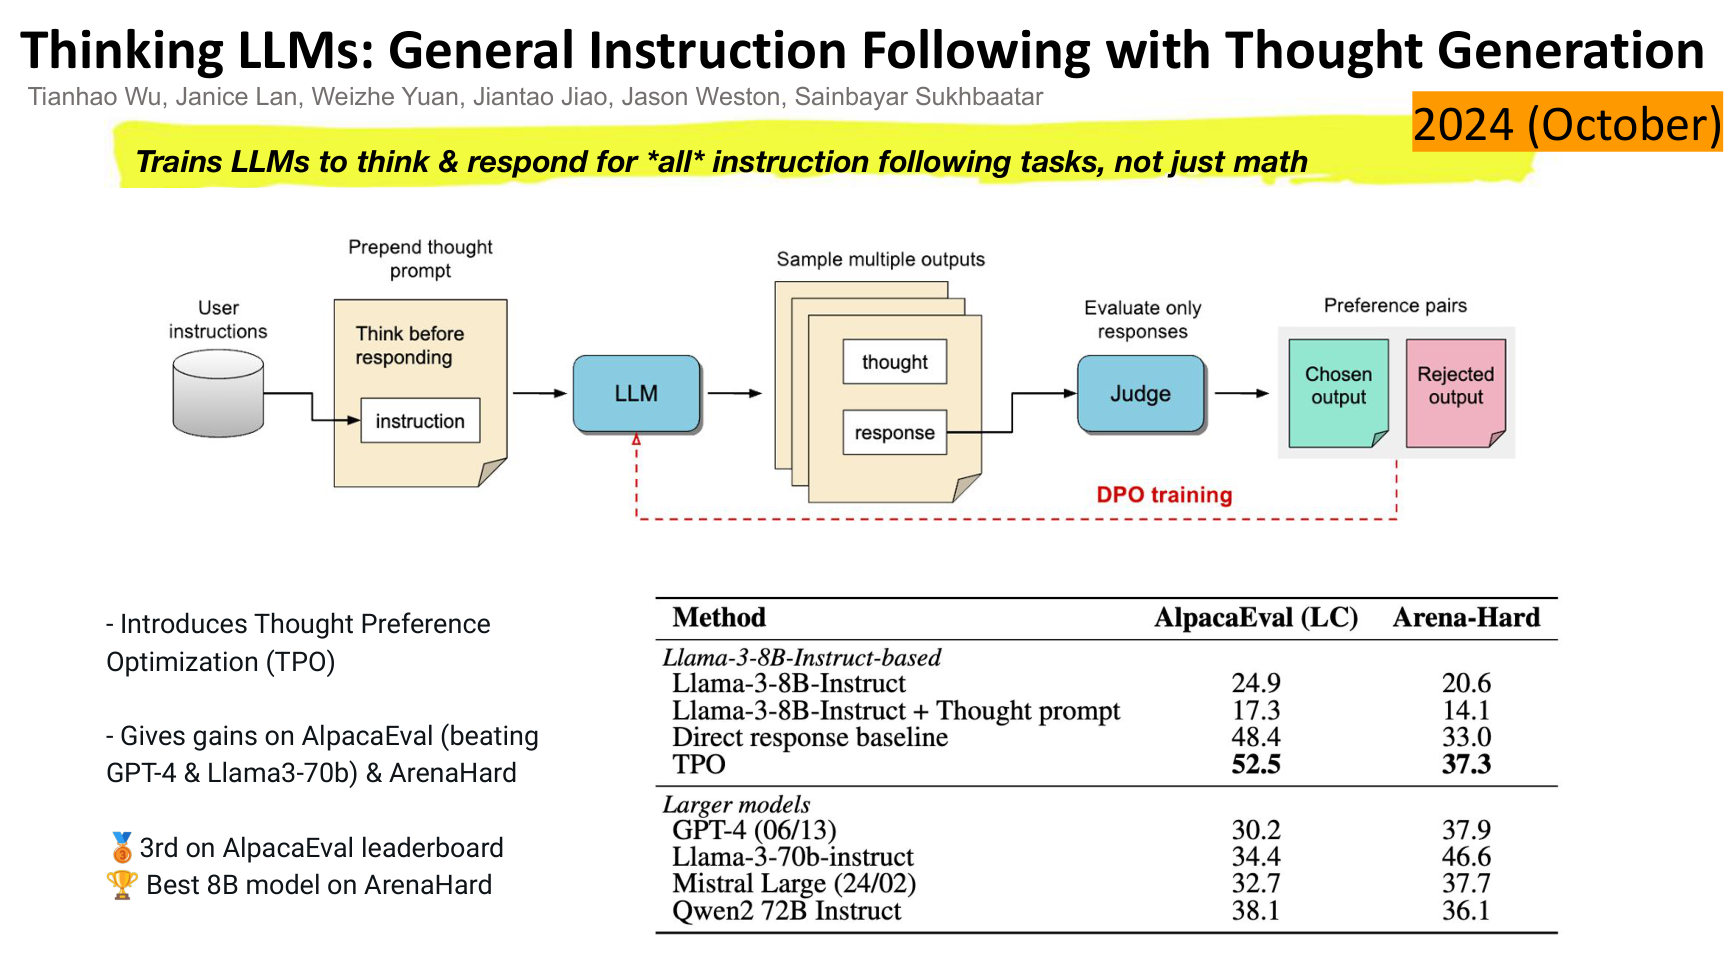
\includegraphics[width=0.76\textwidth]{../lectures/lec02_learning_to_reason/figures/lec02_fig_010.png}
\caption{Thinking LLMs 的主张：thought generation 应该成为更广泛 instruction following 的默认能力，而不是 reasoning benchmark 的特例。}
\end{figure}

这里的关键不是“每道题都写一长串想法”，而是让模型学会何时需要显式计划、何时只需快速回答。对 agent 来说，这意味着 reasoning policy 也应该被训练，而不仅是 final answer style。

\subsubsection{Meta-Rewarding：judge 也要继续被训练}

如果 self-rewarding 把 actor 和 judge 放进同一个模型，下一步自然是：\textbf{judge 本身怎么变强？} Meta-Rewarding 的回答是，让模型不仅学习回答，还学习对 judgment 进行 meta-judgment。

\begin{figure}[H]
\centering
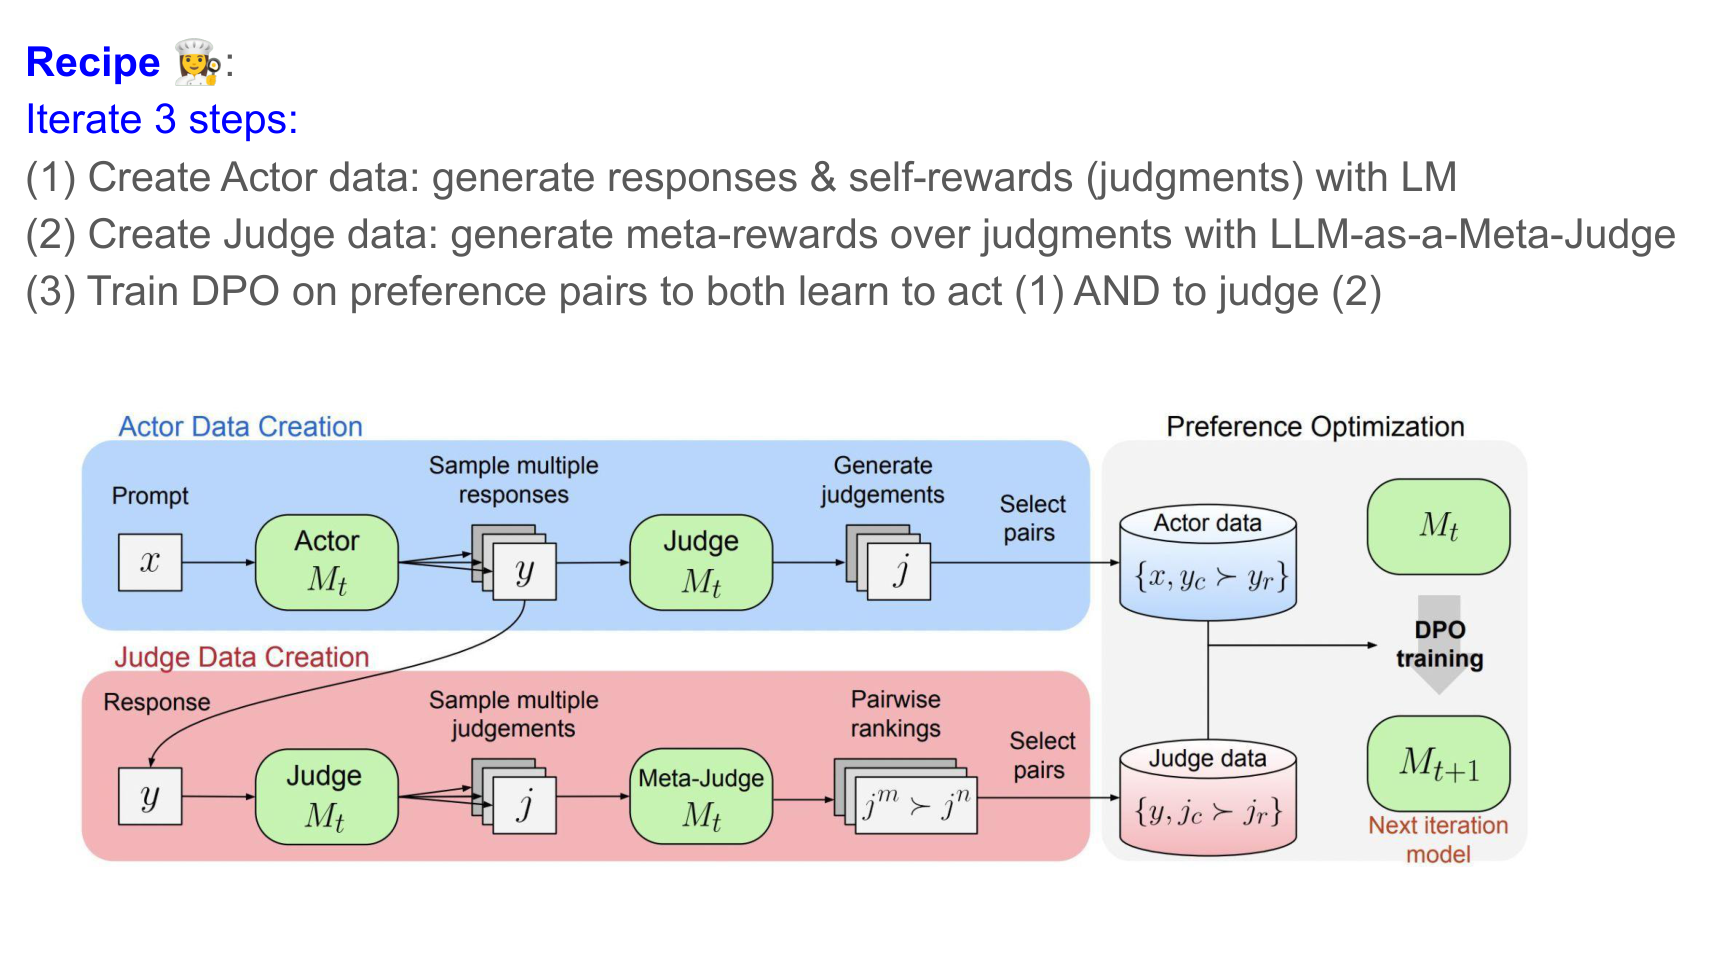
\includegraphics[width=0.78\textwidth]{../lectures/lec02_learning_to_reason/figures/lec02_fig_011.png}
\caption{Meta-Rewarding 的三步循环：生成 actor data、生成 judge data、同时训练 actor 与 judge。}
\end{figure}

一个简化的写法是：
\[
p(i \succ j)=\sigma(s_i-s_j)
\]
其中 $s_i$ 和 $s_j$ 是两个 judgments 的 latent score，$\sigma$ 把分差转成偏好概率。Lecture 用 Elo-style intuition 说明：如果能比较 judgment 本身谁更好，我们就能反过来训练更强的 judge。

\begin{lstlisting}
Create actor data: responses plus self-judgments
Create judge data: meta-judge comparisons over those judgments
Train DPO objectives for both the actor and the judge
\end{lstlisting}

Meta-Rewarding 的价值在于，它直面了“judge 会不会比 actor 落后”的问题。许多系统失败，不是因为生成器不会说，而是因为筛选器不会选。Weston 的路线是把筛选器也当成要持续学习的对象。

\subsubsection{EvalPlanner：让 judge 先计划再打分}

最后，EvalPlanner 把同样的想法推到 evaluation task 上：若评估本身也很难，那么 judge 也应该有自己的 chain-of-thought、planning 和可验证训练数据。

\begin{figure}[H]
\centering
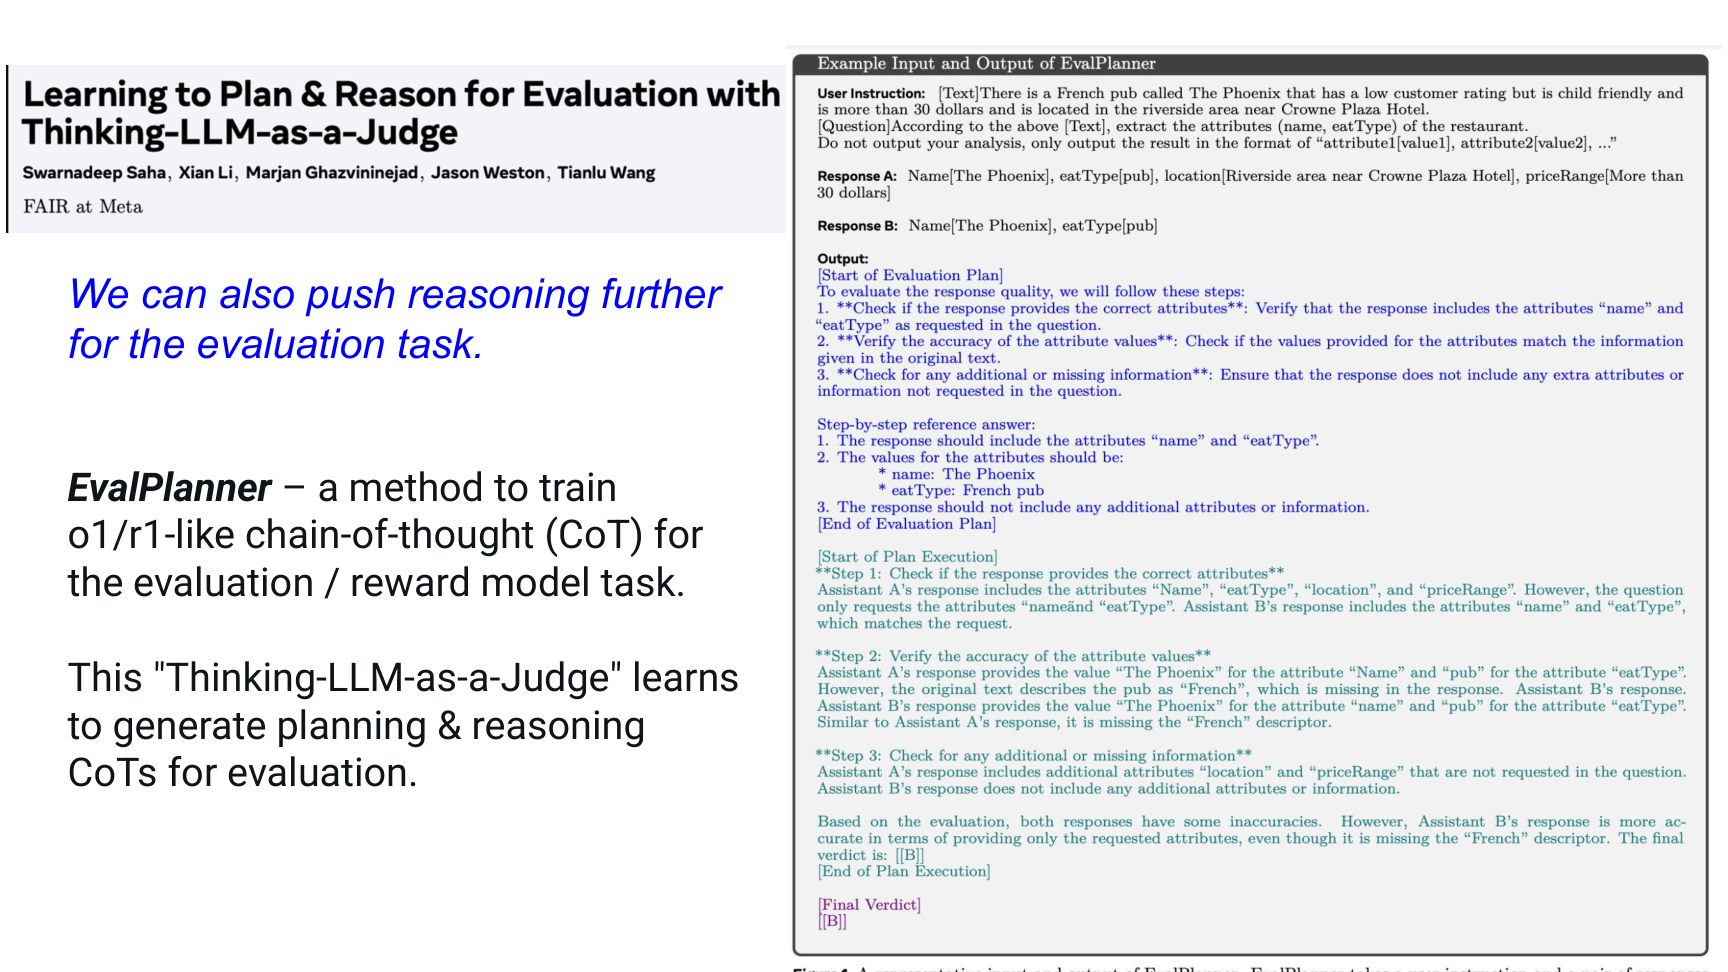
\includegraphics[width=0.78\textwidth]{../lectures/lec02_learning_to_reason/figures/lec02_fig_012.png}
\caption{EvalPlanner 把 evaluation task 转成可验证推理任务，训练的是“会规划的 judge”。}
\end{figure}

\begin{lstlisting}
Generate a good response y to prompt x
Perturb x into a similar prompt x' and generate y'
Convert the pair into a verifiable evaluation task
Train a thinking judge to plan before scoring
\end{lstlisting}

这一步非常关键。到这里，本讲已经把 reasoning learning 的难点重新表述为：\textbf{谁来给出足够好的 reward / judgment，以及这个 reward model 自身如何学习。}

\section{关键公式、算法与 readings 的连接}

\subsection{DPO：本讲所有 recipe 的优化执行器}

DPO reading 之所以重要，不是因为它单独就解决了 reasoning，而是因为它把“有偏好对就能训练”的这件事做得足够简单稳定。Weston 的系统几乎都默认用 DPO 或其变体做最后的优化，因此如果读者忽略 DPO，就会误以为这些方法的创新在于 loss 本身；实际上，创新更常在于\textbf{偏好对是如何被构造出来的。}

\subsection{IRPO：从 response preference 走向 reasoning preference}

IRPO reading 正好补上了 lecture 的核心转折。它证明 reasoning task 上最大的痛点不是“没有 preference optimization”，而是“没有 reasoning-aware preference pairs”。一旦 final answer 可验证，就可以把 CoT 也纳入 preference learning。

\subsection{CoVe：验证先于自信}

CoVe reading 在本讲里承担的是“方法论校正”的角色。它提醒我们，面对 hallucination 问题时，最重要的未必是生成更多候选，而是把 verification workflow 明确写出来，让模型先问“我该如何检查自己”。

\section{失败模式、边界条件与前后讲联系}

\subsection{本讲最重要的失败模式}

\begin{enumerate}
\item \textbf{把 self-rewarding 理解成“模型随便给自己打分”。} 没有可解释 criteria 和种子 judge 数据时，这会迅速漂移。
\item \textbf{把 DPO 当成 reasoning 的全部。} DPO 只是优化器；如果 winning/losing pairs 不携带真实 reasoning signal，它只会学到风格偏好。
\item \textbf{把 CoVe、S2A 当成更长 CoT。} 这些方法真正关心的是验证结构，而不是 token 数。
\item \textbf{在没有可验证 final answer 的任务上直接照搬 IRPO。} 一旦 reward grounding 变弱，reasoning preference 就会变得不可靠。
\item \textbf{忽略 judge 的学习问题。} 很多 agent pipeline 只训练 actor，却让 evaluator 原地踏步，这会导致系统上限卡死。
\end{enumerate}

\subsection{与前后讲的联系}

第一讲讨论的是 inference-time compute 的分配：如何在推理时生成、筛选、修正 reasoning traces。本讲则把焦点移到 training time：如何\textbf{让模型在训练中习得这些 reasoning / judging 行为。} 下一讲 Yu Su 会进一步把 reasoning 放进 language agent 框架，讨论 memory、planning、world model 等结构能力。这意味着课程主线正在从“如何让单个模型更会想”扩展到“如何让 agent 系统在外部环境中更会记、更会规划、更会行动”。

\section{本章小结}

\begin{figure}[H]
\centering
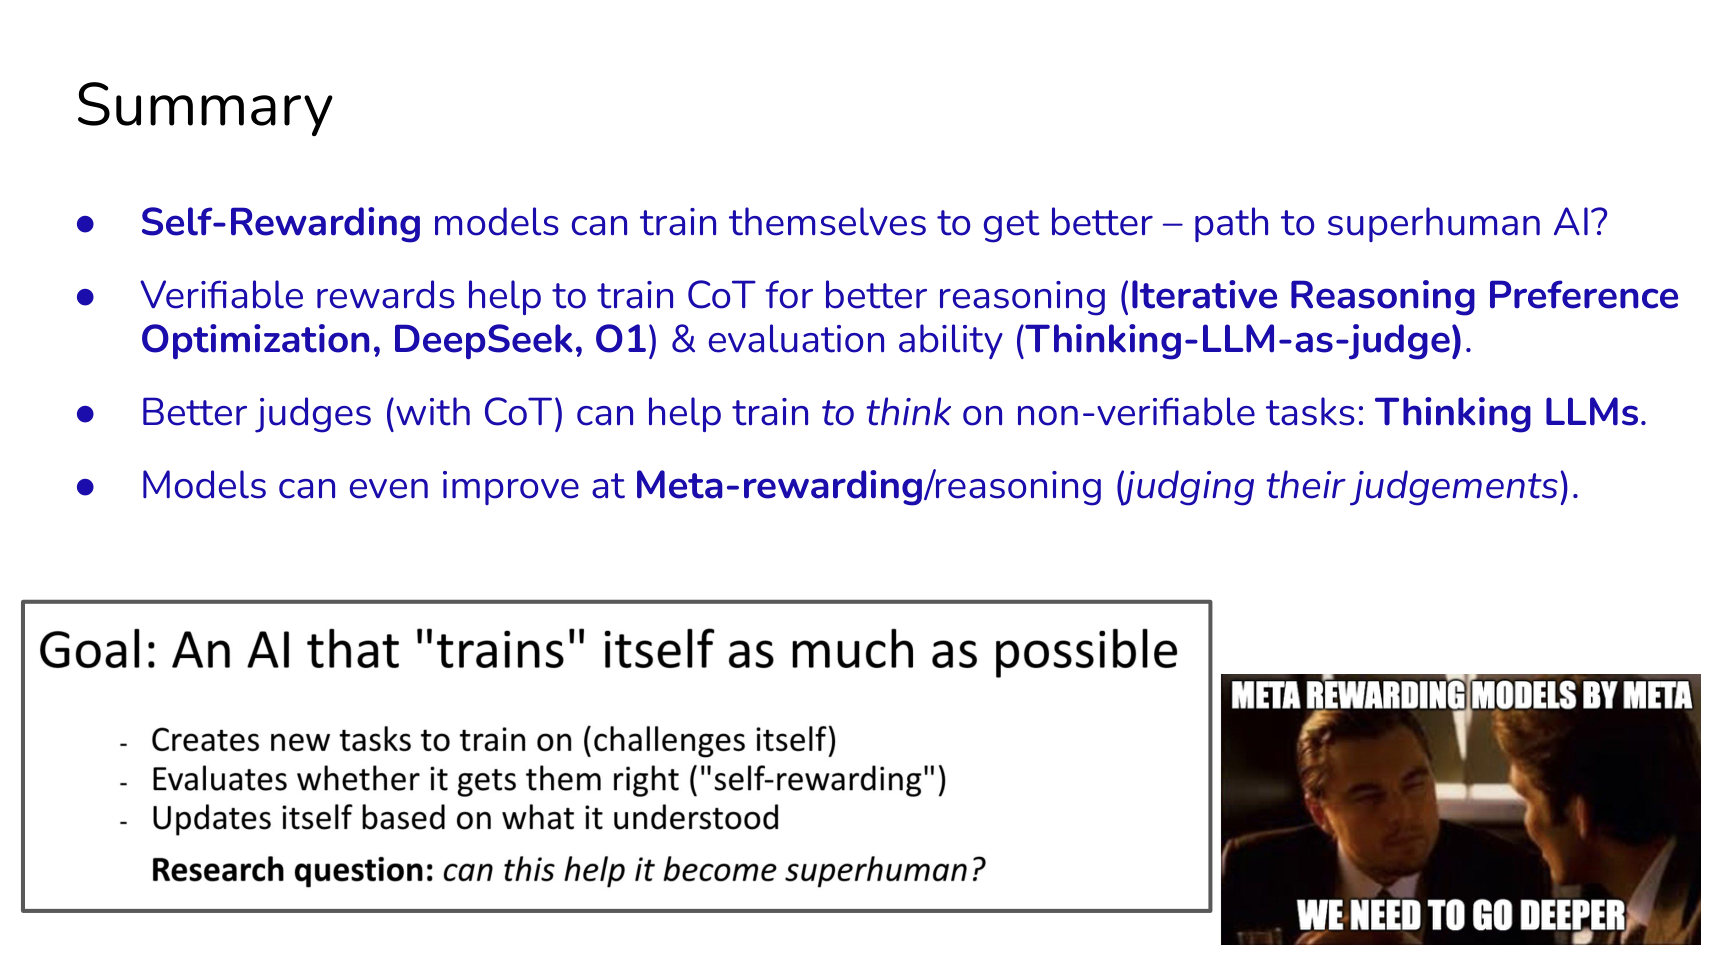
\includegraphics[width=0.76\textwidth]{../lectures/lec02_learning_to_reason/figures/lec02_fig_013.png}
\caption{本讲 summary：reasoning learning 的升级路线，最终都回到了 reward / judgment 是否足够可靠。}
\end{figure}

Weston 这讲最大的贡献，是把“learning to reason”重新写成了“learning to generate better judgments”。其逻辑链条非常清楚：
\begin{itemize}
\item LLM 的 System 1 失败暴露了显式验证与去偏的必要性。
\item 标准 RLHF 的 humans-in-the-loop 无法无限扩展。
\item Self-Rewarding 让 actor 和 judge 一起成长。
\item IRPO 说明 reasoning task 需要可验证 final answer 和 reasoning-specific preference pairs。
\item Meta-Rewarding 与 EvalPlanner 进一步指出：judge 本身也是需要 reasoning 和训练的对象。
\end{itemize}

如果把本讲压缩成一句话，那就是：
\begin{center}
\emph{要让模型学会推理，先得让系统学会更可靠地判断什么才算好的推理。}
\end{center}

\section{复习题}

\begin{enumerate}
\item Weston 为什么把 hallucination、sycophancy、jailbreaking 都归为 System 1 failure？
\item CoVe 与单纯多采样 CoT 的核心差别是什么？
\item DPO 为什么只是 reasoning learning 的“执行器”，而不是完整答案？
\item Self-Rewarding 模型为什么必须同时提升 acting 和 judging 两种能力？
\item IRPO 为什么需要 verifiable final answer 与 negative examples？
\end{enumerate}

\section{深入思考题}

\begin{enumerate}
\item 如果一个任务没有明确 final answer，只能得到模糊的人类评分，你会怎样改写 IRPO 的 reward grounding？
\item Meta-Rewarding 是否会陷入“judge judge judge”的无限回归？系统需要在哪一层停下来并重新接入外部 ground truth？
\item 对真实 agent 环境而言，judge 最终应该主要依赖静态 benchmark、环境反馈，还是人类交互？为什么？
\end{enumerate}

\section{延伸阅读}

\begin{itemize}
\item \textbf{DPO}：理解为什么 KL-constrained RLHF 可以直接化为 preference optimization。
\item \textbf{IRPO}：理解 reasoning preference pair 的构造方式，以及为什么 NLL 项不能轻易拿掉。
\item \textbf{CoVe}：理解 verification planning 在 factuality 问题中的作用。
\item 如继续深入本门课，可将本讲与第一讲的 verifier、Self-Debugging，以及后续 memory / planning 章节一起阅读，形成“生成-评价-修正”的统一视角。
\end{itemize}
